\chapter{Clustering Pipeline} \label{ch:methodology}

To analyze vehicle behavior, we have designed an information fusion pipeline, which divides the analysis into different stages. Each stage fulfills its own objective of data processing and extraction of information that will be relevant in the subsequent stage. In general, the pipeline begins with the extraction and collection of data from heterogeneous sources and finally produces a grouping result from a clustering model based on the decisions we make along the pipeline (see in \cref{fig:arquitectura}). The technologies used to implement and execute the different stages of the pipeline come from the fields of ML and data analysis. In \cref{tab:pipeline-tab}, we can visualize a description of the different stages proposed in the pipeline and the experimental values considered in each of them. The pipeline consists of the following stages: data collection, data cleaning, data fusion, preprocessing, dimension reduction, clustering, evaluation, and visualization. 

\begin{figure}
\begin{center}
	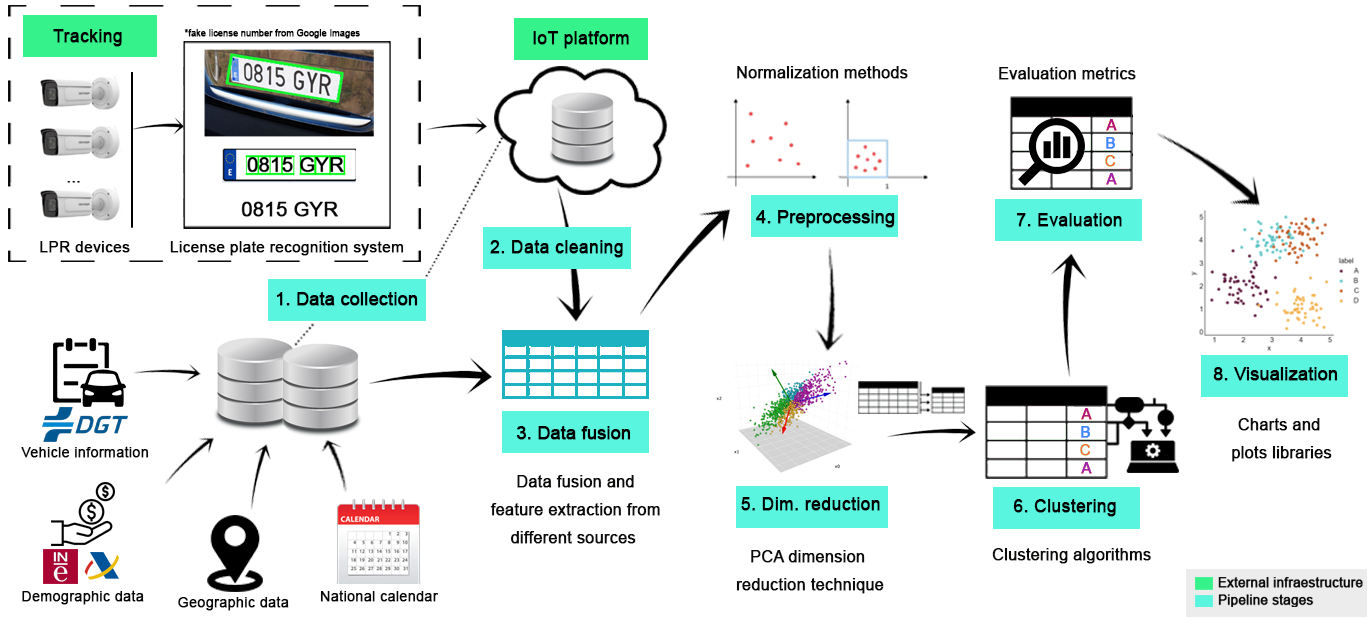
\includegraphics[width = \linewidth]{Images/arquitectura.png}
\end{center}
	\caption{\label{fig:arquitectura} Overview of the clustering pipeline.}
\end{figure}

% Please add the following required packages to your document preamble:
% \usepackage{graphicx}
\begin{table}[]
\centering
\resizebox{\columnwidth}{!}{%
\begin{tabular}{ccc}
\hline
Stage               & Configuration parameters       & Experimental values                                                                                                                                             \\ \hline
Data Collection         & \begin{tabular}[c]{@{}c@{}}Data collection \\ from different sources   \end{tabular}             & \begin{tabular}[c]{@{}c@{}}Storage in own DB and \\ external IoT platform \end{tabular}
                                                \\ \hline
Data Cleaning         & \begin{tabular}[c]{@{}c@{}}Recovery and treatment \\ of lost data   \end{tabular}                & \begin{tabular}[c]{@{}c@{}}1. License plate matching \\ 2. Recover movement of vehicles not \\ detected by any camera in their total route\end{tabular}
\\ \hline
Data Fusion         & \begin{tabular}[c]{@{}c@{}}Fusion of information data \\ and feature extraction   \end{tabular}                & Detailed process in \cref{tab:data-fusion-process}                                                                                                                                                    \\ \hline
Preprocessing       & Normalization methods          &  \begin{tabular}[c]{@{}c@{}}Min-max normalization, z-score standarization, \\ MAD normalization, $\ell^2$ normalizacion        \end{tabular}                                                                                                                                                  \\ \hline
Dimension reduction & \begin{tabular}[c]{@{}c@{}}Dimension reduction \\ techniques \end{tabular} & Principal Component Analysis (PCA)                                                                                                                                                                     \\ \hline
Clustering          & Clustering algorithms          & \begin{tabular}[c]{@{}c@{}}K-Means, MiniBatchKMeans, \\ Agglomerative clustering, BIRCH, \\ DBSCAN, HDBSCAN, MeanShift, \\ Gausian Mixture, Spectral Clustering        \end{tabular}                                                                                                                                                                    \\ \hline
Evaluation          & Evaluation metrics             & \begin{tabular}[c]{@{}c@{}}Silhouette, Davies–Bouldin, \\ Calinski–Harabasz, number of clusters, \\ Bayesian Information Criterion,\\ Akaike Information Criterion\end{tabular} \\ \hline
Visualization       & Visualization plots        & \begin{tabular}[c]{@{}c@{}}box plot, scatter-plot, \\ elbow method, PCA variance plot        \end{tabular}                                                                                                                                                      \\ \hline
\end{tabular}%
}
\caption{Configuration of each stage of the pipeline with the values used in this study.}
\label{tab:pipeline-tab}
\end{table}

\section{Data collection} 
\label{sec:DataCollection}
 The data collection phase handles the collection and storage of our different data sources. This process involves collecting data from different sensors and other data sources, such as Web pages or databases. In our case, we collected the data from LPR cameras and from specific databases we collected: vehicle information, demographic and economic, national calendar, and geographic data.

Regarding vehicle tracking infrastructure (LPR cameras), data is collected by four devices equipped with vehicle detection sensors. These devices are Hikvision LPR IP cameras with Automatic number-plate recognition (ANPR) based on Deep Learning. The devices have a 2MP resolution, 2.8-12 mm varifocal optics, and IR LEDs with a range of 50 m.

To cover the entrances and exits of each village in the target area, we strategically positioned the four cameras, as shown in \cref{fig:map}. The locations are (i) entrance to Pampaneira from the western part of the Alpujarra, (ii) entrance to Pampaneira from the eastern part of the Alpujarra, (iii) entrance to Bubión via a single road, and (iv) entrance to Capileira via a single road. By taking advantage of the road structure, we can monitor the mobility of all vehicles that circulate in the Poqueira area using only four LPRs.

\begin{figure}
\begin{center}
	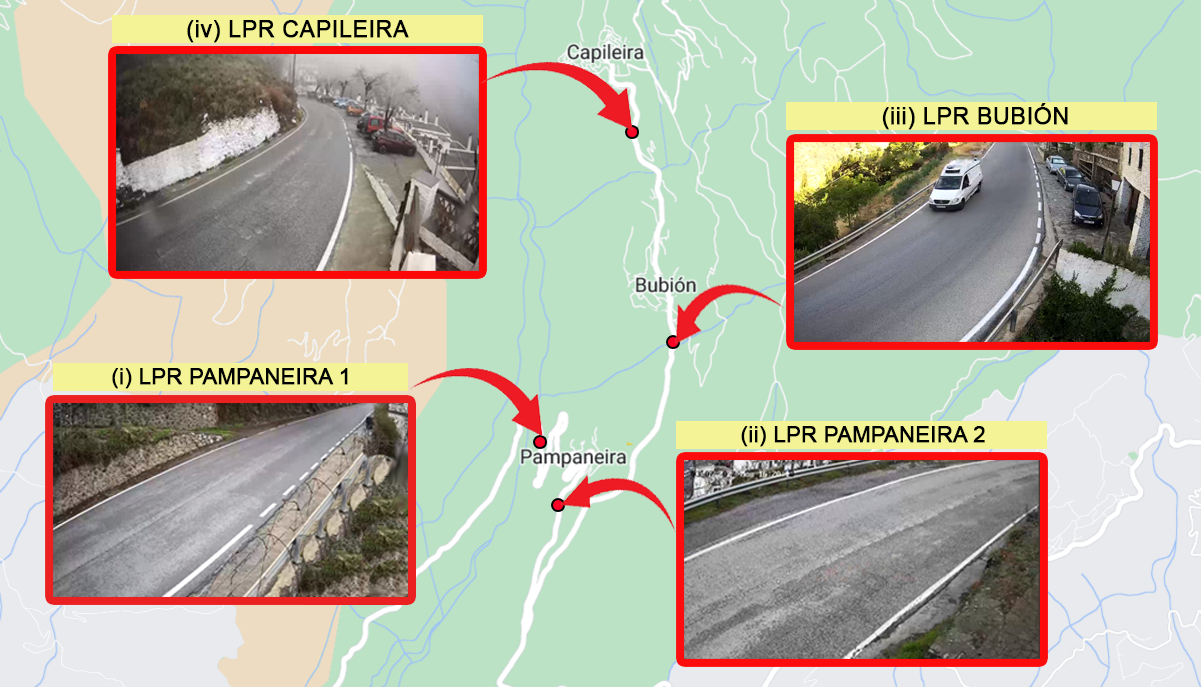
\includegraphics[width = \linewidth]{Images/setup_map.png}
\end{center}
	\caption{\label{fig:map} Setup of the 4 LPR that obtain the data from the license plates of the vehicles.}
\end{figure}

The main objective of these cameras is to track vehicles entering and leaving each of the villages, providing detailed knowledge of mobility in the Poqueira area. Using only four cameras also helped minimize the cost and complexity of the system while still capturing the necessary data. The information collected by the cameras is stored on a cloud platform.

The rest of the data were collected from different databases. Vehicle information from a private dataset of the National Traffic Department. The demographic and economic information from the Internet website of the National Statistics Institute and the Tax Agency. the national calendar and the geographic data are from Python libraries.  


\section{Data Cleaning} 
\label{sec:DataCleaning}
In the field of the IoT, the production of sensor data can often be inaccurate and lead to the loss of some records. In our case, we present two cleaning steps for the main dataset (LPR cameras). The first step, ``license plate matching", aims to reduce the error rate of incomplete or wrongly detected license plates by the LPR devices to maintain consistency between vehicles with the same license plate. About 2\% of the stored 1,050,760 records have missing values in the license plate number. For example, if we have a record with a correct license plate 0000AAA, and another record with the value 0\#00AAA, missing the second digit, we could, by probability, infer that both records belong to the same plate number and assign the correct value, 0000AAA, to both records. In our case, we assign the same plate number to all those records whose license plate matches at least four characters out of seven in the same position. The second step, ``route recovery", aims to reduce the percentage of vehicles not detected by any LPR device. These errors occur when the camera does not detect a vehicle that passes through the road. This error is difficult to detect, but in our setup, if a vehicle moves on the road from camera 1 to 3, and camera 2 (in the middle of the unique road connecting cameras 1 and 3), does not detect the car, we could infer that the car has passed through camera 2. In our process, if the vehicle is detected in less than 30 minutes in two non-consecutive cameras, our system infers that the vehicle is still in the area and calculates its time of stay based on the new registered values.

\section{Data Fusion} \label{sec:DataFusion}

The area where we conducted the experiments, as presented in Section \ref{sec:smartvillages}, records individuals with diverse behavioral patterns and experiences a large flow of tourists from different parts of Spain and elsewhere, each with unique mobility characteristics that vary by region of provenance. Combining data from provenance, mobility in the area, and the holiday calendar offers the opportunity to gain an understanding of the region, its inhabitants, and visitors. This section explains each source of information and the feature extraction and construction process of each dataset to allow the merging. We will detail the structure and variables obtained for each data source, creating a joint database. \cref{tab:data-fusion-process} schematically shows the information fusion process we have followed.


% Please add the following required packages to your document preamble:
% \usepackage{graphicx}
\begin{table}[]
\centering
\resizebox{\columnwidth}{!}{%
\begin{tabular}{lll}
\hline
\multicolumn{1}{c}{Phase} &
  \multicolumn{1}{c}{Tasks} &
  \multicolumn{1}{c}{Values} \\ \hline
\multicolumn{3}{c}{Calendar Data} \\ \hline
Importing Data &
  \begin{tabular}[c]{@{}l@{}}Read the dataset with information on \\ public holidays at national level in Spain\end{tabular} & \begin{tabular}[c]{@{}l@{}}270 days, 3 attributes \\ (date, type, holiday\_period) \end{tabular} \\ \hline
\begin{tabular}[c]{@{}l@{}}Set holiday \\ periods\end{tabular} &
  \begin{tabular}[c]{@{}l@{}}Establish the important holiday \\ periods in Spain: Summer Holiday, \\ Christmas and Holy Week\end{tabular} &
  \begin{tabular}[c]{@{}l@{}}Summer Holiday (from 1 aug. to 31 aug.)  \\ Christmas (from 12 dec. to 6 jan.)\\ Holy Week (from 10 apr. to 17 apr.)\end{tabular} \\ \hline
  \begin{tabular}[c]{@{}l@{}} Encode variables\end{tabular} &
  \begin{tabular}[c]{@{}l@{}}Convert categorical holiday periods \\ into binary variables\end{tabular} & \begin{tabular}[c]{@{}l@{}}270 days, 5 attributes \\ (date, type, Summer, Christmas, Holy\_Week) \end{tabular} \\ \hline
\multicolumn{3}{c}{License Plate Recognition Data} \\ \hline
Importing Data &
  \begin{tabular}[c]{@{}l@{}}Read the cleaned dataset produced \\ from the detection of vehicle license plates \end{tabular} &\begin{tabular}[c]{@{}l@{}}
  1,050,760 rows, 4 attributes \\ (license\_plate, time\_stamp, type, camera\_id)\end{tabular} \\ \hline
\begin{tabular}[c]{@{}l@{}}Calculate \\ associate variables\end{tabular} &
  \begin{tabular}[c]{@{}l@{}}Calculate variables combining the 4 cameras\end{tabular} & \begin{tabular}[c]{@{}l@{}}(license\_plate, entry\_time\_stamp, exit\_time\_stamp, \\ route, total\_distance)\end{tabular}
   \\ \hline
Group information &
  Group the information for each record by vehicle & \begin{tabular}[c]{@{}l@{}}50,901 rows, 10 attributes \\ (license\_plate, total\_entries, avg\_visit\_POQ, \\ std\_visit\_POQ, total\_time\_POQ, nights, route, \\ total\_distance, visits\_dif\_weeks, visits\_dif\_months)\end{tabular}
   \\ \hline
\multicolumn{3}{c}{Vehicle information Data} \\ \hline
Importing Data &
  \begin{tabular}[c]{@{}l@{}}Reads the dataset with vehicle \\ information and its origin\end{tabular} & \begin{tabular}[c]{@{}l@{}}
  45,132 license plates, 4 attributes \\ (license\_plate, postcode, co2\_emissions, num\_seats) \end{tabular} \\ \hline
\multicolumn{3}{c}{Demographic and Economic data} \\ \hline
Importing Data &
  \begin{tabular}[c]{@{}l@{}}Reads demographic information about \\ the region of origin of the vehicle\end{tabular} & \begin{tabular}[c]{@{}l@{}}
  11,752 regions, 4 attributes \\ (postcode, population, gross\_income, disposable\_income)\end{tabular} \\ \hline
  Merging Data &
  \begin{tabular}[c]{@{}l@{}}Merge the two sources \end{tabular} & INE
   \\ \hline
   Validate Data &
  \begin{tabular}[c]{@{}l@{}}Validate information \\ common to the two sources\end{tabular} & INE
   \\ \hline
\multicolumn{3}{c}{Geographic data} \\ \hline
Importing Data &
  \begin{tabular}[c]{@{}l@{}}Reads information regarding the \\ region of origin of the vehicle\end{tabular} &
   \begin{tabular}[c]{@{}l@{}}
  11,752 regions, 8 attributes \\ (postcode, autonomous\_community, province, \\ county, district, town, latitude, longitude)\end{tabular} \\ \hline
    Merging Data &
  \begin{tabular}[c]{@{}l@{}}Mix and validate information \\ from the two sources used\end{tabular} & geopy and pgeocode
   \\ \hline
Standardize values &
  \begin{tabular}[c]{@{}l@{}}Treatment of equivalences between names \\ of regions in different co-official languages\end{tabular} & \begin{tabular}[c]{@{}l@{}}Elimination of accents, spaces and translation \\ to Spanish of all values related to region names\end{tabular}
   \\ \hline
Validate Data &
  \begin{tabular}[c]{@{}l@{}}Validate postcodes and geolocation\end{tabular} & geopy, pgeocode and INE
   \\ \hline
\begin{tabular}[c]{@{}l@{}}Generate \\ new variables\end{tabular} &
  \begin{tabular}[c]{@{}l@{}}Calculate the distance between the study area \\ and the postcode origin from the coordinates\end{tabular} &\begin{tabular}[c]{@{}l@{}}
  11,752 regions, 9 attributes \\ (postcode, autonomous\_community, province, \\ county, district, town, latitude, longitude, km\_to\_POQ)\end{tabular} \\ \hline
\multicolumn{3}{c}{Fusion Dataset} \\ \hline
Merging Data &
\begin{tabular}[c]{@{}l@{}}Unification of header names and data formats, \\Mix postcode and license plate fields, \\Delete rows with some null fields\end{tabular}
   &
  \begin{tabular}[c]{@{}l@{}}
  49,224 vehicles, 24 attributes \\ (license\_plate, total\_entries, avg\_visit\_POQ, std\_visit\_POQ, \\ total\_time\_POQ, nights, route, total\_distance, \\ visits\_dif\_weeks, visits\_dif\_months, co2\_emissions, num\_seats, \\ postcode, autonomous\_community,  province, county, \\ district, town, latitude, longitude, km\_to\_POQ, \\ population, gross\_income, disposable\_income)\end{tabular} \\ \hline 
  \begin{tabular}[c]{@{}l@{}}Generate \\ new variables\end{tabular} &
  \begin{tabular}[c]{@{}l@{}}Calculate variables related to the type \\ of dates in the calendar during the period \\ of stay of each vehicle\end{tabular} & \begin{tabular}[c]{@{}l@{}}
  49,224 vehicles, 29 attributes \\ (license\_plate, total\_entries, avg\_visit\_POQ, std\_visit\_POQ, \\ total\_time\_POQ, nights, route, total\_distance, \\ visits\_dif\_weeks, visits\_dif\_months, co2\_emissions, num\_seats, \\ postcode, autonomous\_community,  province, county, \\ district, town, latitude, longitude, km\_to\_POQ, \\ population, gross\_income, disposable\_income, \\ total\_holiday, total\_workday, entry\_in\_holiday,\\ total\_high\_season, total\_low\_season)\end{tabular}
   \\ \hline
Exporting Data &
  Obtaining the resultant dataset & CLUSTERING\_VEHICLES DB
  \\ \hline
\end{tabular}%
}
\caption{Detailed schematic of the data fusion stage in the pipeline.}
\label{tab:data-fusion-process}
\end{table}


\subsection*{License Plate Recognition Data} \label{subsec:setup}

The LPR cameras described in Section \ref{sec:DataCollection} return information on four variables: the vehicle license plate (license\_plate), the time stamp (time\_stamp), and the direction (type) for each camera defined by an identifier (camera\_id). The dataset contains information for nine months (February to October 2022). On these data, we perform the data cleaning that we defined in Section \ref{sec:DataCleaning}. We change the original license plate value to an integer value that functions as the vehicle identifier. In total, we have 1,050,760 records, of which 25.69\% correspond to the camera PAMPANEIRA 1 (i), 29.25\% to PAMPANEIRA 2 (ii), 19.16\% to BUBION (iii) and 25.9\% to CAPILEIRA (iv) (see in \cref{fig:map}). We grouped the records based on the new vehicle identifier (num\_plate\_ID), taking into account the mobility behavior of each vehicle. For each vehicle, we built a record per each time the vehicle visits the area, containing the date of entry (entry\_time\_stamp) and exit (exit\_time\_stamp) to the area and a list of all the cameras (route) by which it has been registered during its stay, from which we can calculate the distance in kilometers traveled (total distance) in the area. From the above records, we can also calculate the duration of stay (avg\_visit\_POQ) expressed in days and the number of nights spent there. In case of missing data, i.e., we cannot calculate the time of entry or exit of a vehicle in the area, we remove the individual from the dataset.

After that, we performed a grouping at the license plate level so that each database row corresponds to a different individual. In this way, we fuse the information of all the vehicle visits in the area. Finally, we obtained a dataset with the total number of visits (total\_entries), the average time (avg\_visit\_POQ) in days, the complete vehicle routing (route), the total accumulated distance traveled (total\_distance), the standard deviation of the average time of each visit (std\_visit\_POQ) in days, the total time spent (total\_time\_POQ) in the area and the total number of nights spent there (nights). From the new record structure, we can calculate the visits of each vehicle in different weeks (visits\_dif\_weeks) and months (visits\_dif\_months) to study the fidelity of the individual in the area. Finally, we obtain a dataset with 50,901 vehicle records and ten attributes.

\subsection*{Vehicle Information Data} \label{sec:DGT}

The National Department of Traffic in Spain (DGT) has provided us with data relating to vehicle information\footnote{\url{https://sede.dgt.gob.es/es/vehiculos/informe-de-vehiculo/}} including details such as the vehicle's CO2 emissions (co2\_emissions), the number of seats (num\_seats) and the postcode of the vehicle's address (postcode). It is important to note that each vehicle is associated with a fiscal address used to pay road tax.  This will generally match the place of origin of the vehicle driver, although as we have described in Section \ref{sec:smartvillages}, this is not entirely true. This dataset will help us understand the distribution of vehicle types and ownership in the different regions. We have a dataset with 45,132 vehicles registered in Spain and four attributes. Unfortunately, we do not have this information for vehicles registered outside of Spain. The percentage of foreigners in the data sample is less than 9.5\%. Therefore, we determined these individuals exclusively by their mobility behavior in the area. All information related to vehicle information, demographic, economic, and calendar holidays is restricted to Spanish-registered vehicles.   

\subsection*{Demographic and Economic data}

We have access to data regarding population size (population), average gross income (gross\_income), and average disposable income (disposable\_income) per person for each region linked to a postcode (postcode). This information comes from different sources such as the Spanish Tax Agency (AEAT)\footnote{\url{https://sede.agenciatributaria.gob.es/Sede/estadisticas.html}} or the National Statistics Institute (INE)\footnote{\url{https://www.ine.es/dynt3/inebase/es/index.htm?padre=7132\&capsel=5693}}. The data are available for regions with more than 1000 inhabitants and are updated until 2020. When using the AEAT source, we noted that some regions were missing, so we relied solely on the INE as a source for the variables mentioned.  The information collected in this database allows us to understand each region's economic and demographic characteristics, which can be valuable for analyzing patterns in the data related to the drivers' economic capacity and willingness to travel. We obtained a database with 11,752 postcode records from Spain and four attributes. 

\subsection*{National calendar data}

We obtain the holiday data using  a holiday library, which also allows the creation of custom calendars for local holidays, long weekends, and bank holidays. The library is designed to quickly and efficiently generate holiday sets specific to each country and subdivision (such as state or province)\footnote{\url{https://python-holidays.readthedocs.io/en/latest/}}. It aims to determine whether a particular date is a public holiday and to set national and regional holidays for multiple countries. As we mentioned before, due to the small percentage of foreign individuals in the sample, and the complexity of dealing with a different set of holidays for different vehicles, we have restricted the analysis of the holidays to Spain. However, in the holidays, we include Saturdays and Sundays, so we also consider the idea of a weekly holiday for any origin. For each day, represented by a date (date), we have information (type) on whether it is a holiday or a working day in Spain. In addition, holiday periods have been defined to establish high and low tourist seasons based on the three most important national holidays in Spain: Summer, Christmas, and Holy Week\footnote{\url{https://es.statista.com/temas/3585/vacaciones-en-espana/\#topicOverview}}, which represent a binary variable, indicating whether the date belongs to that holiday period (Summer, Christmas, Holy Week). We obtain a database with 270 days and five attributes.

\subsection*{Geographic data}

We get the geographic origin of the vehicles using the postcode and two libraries: pgeocode and geopy. pgeocode\footnote{\url{https://pgeocode.readthedocs.io/en/latest/}} allows fast and efficient queries of GPS coordinates, region name, and municipality name from postcodes. The library can also calculate the distances between postcodes. geopy\footnote{\url{https://geopy.readthedocs.io/en/latest/}} is a Python client that provides access to several popular geocoding web services. It allows developers to find the coordinates of addresses, cities, countries, and landmarks from third-party geocoders and other data sources. The library includes geocoding classes for numerous services, such as OpenStreetMap Nominatim and Google Geocoding API (V3), which can be found at geopy.geocoders. We use data from both sources to validate and complement each other's vehicle location information at different levels, such as municipality, county, or suburb. Furthermore, we also use data from the National Statistics Institute (INE)\footnote{\url{https://www.ine.es/daco/daco42/codmun/cod\_ccaa\_provincia.htm}} to verify the province and autonomous community code of the vehicle, which is directly related to the postcode. Hence, we have created a database that contains, for each postcode, information about: (autonomous\_community), (province), (county), (district), (town), (latitude), (longitude), and distance in kilometers between the origin of the vehicle and the study area (km\_to\_POQ). We obtain a database with 11,752 postal code records for Spain and nine attributes.

\subsection*{Merge of all the processed datasets}

Finally, we fuse all constructed databases, crossing the information from the license plate and postcode variables. After merging the tables, we eliminated records with any of the aforementioned attributes null. The information from the national calendar allows us to add to the vehicle database information related to the stay and its total number of holidays (total\_holiday), workdays (total\_workday), high season (total\_high\_season), low season (total\_high\_season) and a binary variable indicating whether the vehicle enters the area on a holiday or a workday (entry\_in\_holiday). The resulting dataset contains information on the behavior in the area for 49,224 vehicles and 29 attributes. 

\section{Preprocessing} \label{sec:preprocessing}

Our dataset contains about 29 attributes with different scales and units. Hence, some variables may be more influential than others in our analysis. To solve this problem, we will apply normalization to the data. Normalization must be applied to numerical data, so we must first convert the categorical variables to numerical values. Of the 29 variables, only the following are categorical: postcode, route, autonomous\_community, province, county, district, town, license\_plate. The variable license\_plate is a unique identifier of each record, so we delete it. The region variable directly correlates with the km\_to\_POQ, so we can eliminate this feature without losing information. For the same reason, we eliminated the variables latitude and longitude. The numeric variable, total\_distance, keeps the information of the kilometers traveled in the variable route. We will not use in this problem the variables co2\_emissions and num\_seats, since they contain empty values for a high percentage of individuals (approx. 25\%). Also, we believe that for this problem, they do not provide information of relevant interest. We will finally obtain a dataset with 49,224 vehicles and 17 numerical attributes: total\_entries, avg\_visit\_POQ, std\_visit\_POQ, total\_time\_POQ, nights, total\_distance, visits\_dif\_weeks, visits\_dif\_months, km\_to\_POQ, population, gross\_income, disposable\_income, total\_holiday, total\_workday, entry\_in\_holiday, total\_high\_season, total\_low\_season. 

\section{Dimensionality reduction} 

%After preprocessing, we reduce the dimensionality of the dataset. 
It is advisable to reduce the search space of the feature matrix before the clustering for efficiency reasons. This process aims to create a simplified set of dimensions containing much of the variance of the original dataset, as there could be features with very low variance, which would make them of little use for our goal of clustering into different vehicle behaviors. Specifically, we want to minimize the number of components as a function of the variance explained. Hence, after the normalization in Section \ref{sec:preprocessing}, we apply Principal Component Analysis (PCA), as a dimensionality reduction algorithm. The result of this stage is a projection of the original dimensions onto a smaller number of new dimensions, also called PCA components. Then, we will evaluate which normalization offers a higher variability value on a fixed value of PCA components. Visualizing the variance explained by each component can help choose the best normalization. This analysis will be discussed in Chapter \ref{ch:results}.

Removing highly correlated features can cause a loss of information for data with high dimensionality, and the PCA technique reduces the dimension of the dataset \cite{frost2017multicollinearity}. However, we have found that removing variables with very high correlation substantially improves the results and the performance of the clustering models for our data. Furthermore, correlated variables increase the data's variance, making the visual interpretation of the PCA results difficult, as the firsts principal components may not accurately reflect the underlying structure of the data.

\section{Clustering and evaluation}

Our choice of unsupervised machine learning is motivated by the need to categorize unlabeled individuals into distinct groups. Our study explores all the algorithms mentioned in Section \ref{subsec:algorithms} to determine the optimal approach for pattern recognition and evaluate whether they can find a realistic solution.

\section{Visualization} 

Data visualization is essential in our work, as it helps to determine and make decisions about parameter settings, algorithms, and normalization used in our analysis. Likewise, it helps in the explainability of the machine learning results. Regardless of the metrics used, performing a visual evaluation of the results is recommended. Combining the evaluation metrics and visualization charts, we can reach conclusions that facilitate making informed decisions on configuring our model. For example, we use the elbow method to determine the optimal number of clusters for different algorithms. This method consists of plotting a graph based on the number of clusters or components and a given evaluation metric, and visually looking for the inflection point on the defined curve (``elbow"). By selecting the number of components at the bend, we strike a balance between model complexity and accuracy. 

We have visualized the first two PCA components for each normalization with scatter plots to study the data's geometry and the clusters' distribution. These visualizations help to understand the underlying structure of the data. However, there is a limitation in the number of coordinates supported for the scatter plot (maximum 3). Some graphs, such as the Andrews curves, exceed the theoretical limit of the number of components displayed, as they are based on the Fourier series. The problem arises because too many individuals in the dataset overlap, which causes the cluster curves to overlap as well and, thus, provide limited visual information. Therefore, this graph is not helpful for our data. We also use box plots to visualize the distribution of each feature among the individuals in each generated cluster. By comparing these distributions between different clusters, we can identify common patterns that help us understand the individuals that compose each cluster.